
\chapter{Jet Mass Observable Distribution}
\label{appendixA}
Kinematic distribution for all the samples, $\pt$ $\eta$ and $\phi$ is shown.

\begin{figure}
    \centering
    \begin{subfigure}[b]{0.45\textwidth}
        \includegraphics[width=\textwidth]{/Users/fabnap/Documents/MasterArbeit/jet_part/appendixA/tops/1cfrt_h_FatJet_pt.pdf}
        \caption{$\pt$ distribution}
        \label{fig:gull}
    \end{subfigure}
    \begin{subfigure}[b]{0.45\textwidth}
        \includegraphics[width=\textwidth]{/Users/fabnap/Documents/MasterArbeit/jet_part/appendixA/tops/1cfrt_h_FatJet_eta.pdf}
        \caption{$\eta$ distribution}
        \label{fig:tiger}
    \end{subfigure}
    \begin{subfigure}[b]{0.45\textwidth}
        \includegraphics[width=\textwidth]{/Users/fabnap/Documents/MasterArbeit/jet_part/appendixA/tops/1cfrt_h_FatJet_psi.pdf}
        \caption{$\phi$ distribution}
        \label{fig:mouse}
    \end{subfigure}
    \caption{Boosted tops kinematic distribution.}\label{fig:animals}
\end{figure}


\begin{figure}
    \centering
    \begin{subfigure}[b]{0.45\textwidth}
        \includegraphics[width=\textwidth]{/Users/fabnap/Documents/MasterArbeit/jet_part/appendixA/higgs/1cfrt_h_FatJet_pt.pdf}
        \caption{$\pt$ distribution}
        \label{fig:gull}
    \end{subfigure}
    \begin{subfigure}[b]{0.45\textwidth}
        \includegraphics[width=\textwidth]{/Users/fabnap/Documents/MasterArbeit/jet_part/appendixA/higgs/1cfrt_h_FatJet_eta.pdf}
        \caption{$\eta$ distribution}
        \label{fig:tiger}
    \end{subfigure}
    \begin{subfigure}[b]{0.45\textwidth}
        \includegraphics[width=\textwidth]{/Users/fabnap/Documents/MasterArbeit/jet_part/appendixA/higgs/1cfrt_h_FatJet_psi.pdf}
        \caption{$\phi$ distribution}
        \label{fig:mouse}
    \end{subfigure}
    \caption{RS-Graviton kinematic distribution.}\label{fig:animals}
\end{figure}

\begin{figure}
    \centering
   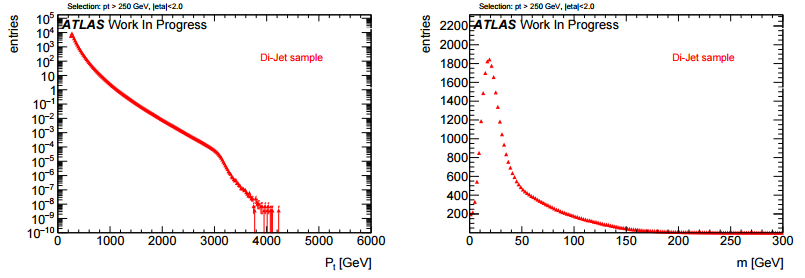
\includegraphics[width=\textwidth]{/Users/fabnap/Documents/MasterArbeit/jet_part/appendixA/qcd/qcdkinematics.png}
   
    \caption{QCD dijet transverse momentum and mass distributions.}
    \label{fig:qcdkinematics}
\end{figure}

\begin{figure}[!ht]
  \centering
      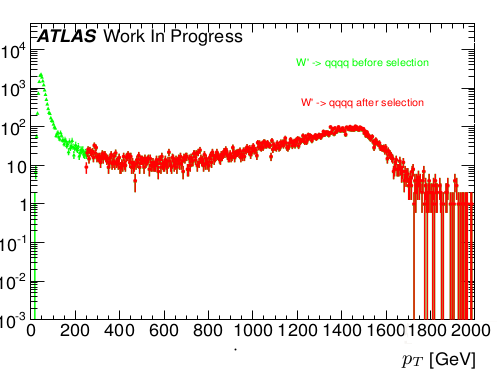
\includegraphics[width=0.5\textwidth]{/Users/fabnap/Documents/MasterArbeit/jet_part/ptjcobian.png}
  \caption{The $\pt$ distribution of a 3 TeV resonance from the hadronically decaying $W$ or $Z$, in logarithmic plot. As can be seen, the jacobian peak is around $\pt\simeq m_{W'}/2\simeq 1.5$ TeV.}
  \label{fig:ptjacobian}
\end{figure}


\begin{figure}
    \centering
    \begin{subfigure}[b]{0.45\textwidth}
	\centering
        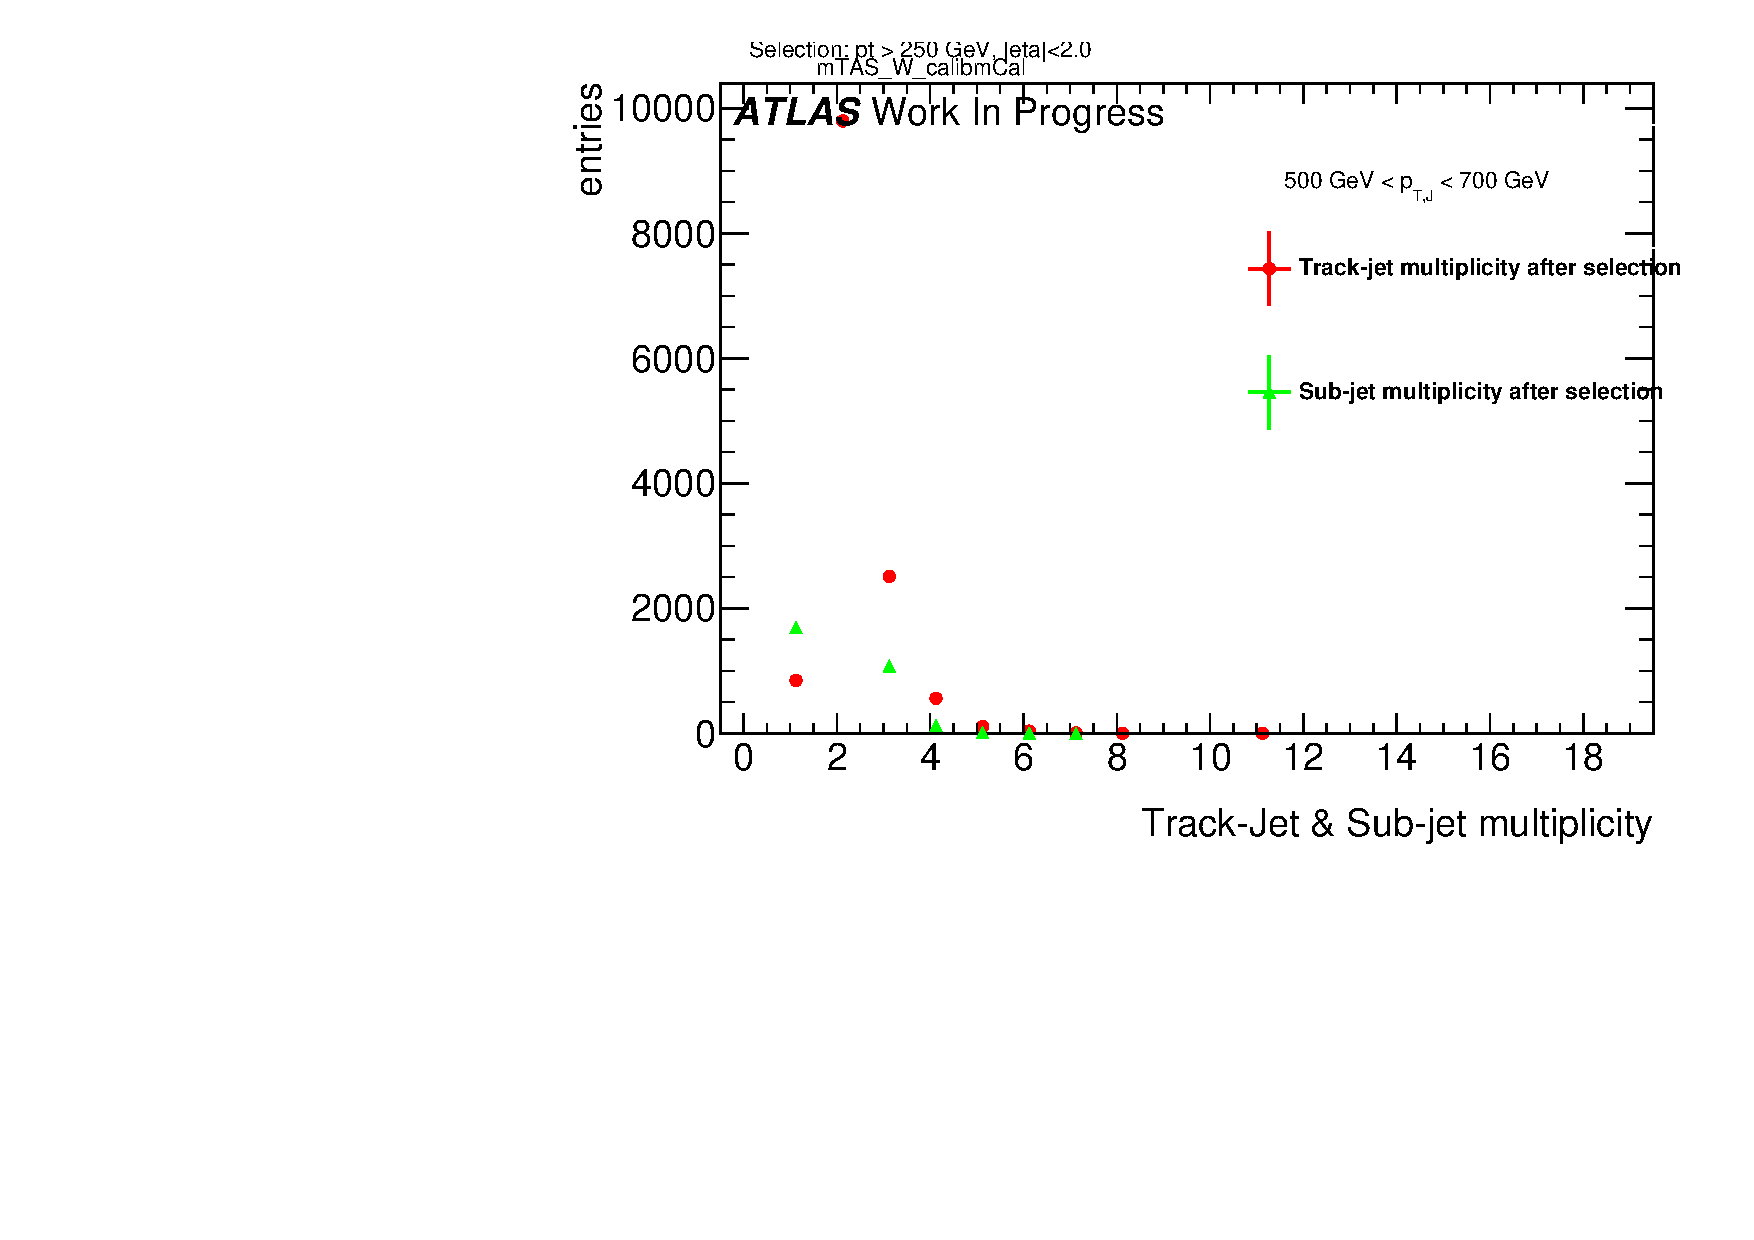
\includegraphics[width=\textwidth]{/Users/fabnap/Documents/MasterArbeit/jet_part/mta/13cfrt_h_SubJet_aftersel_ptJ03TAmult.pdf}
 
%         \label{fig:gull}
    \end{subfigure}
    \begin{subfigure}[b]{0.45\textwidth}
	\centering
        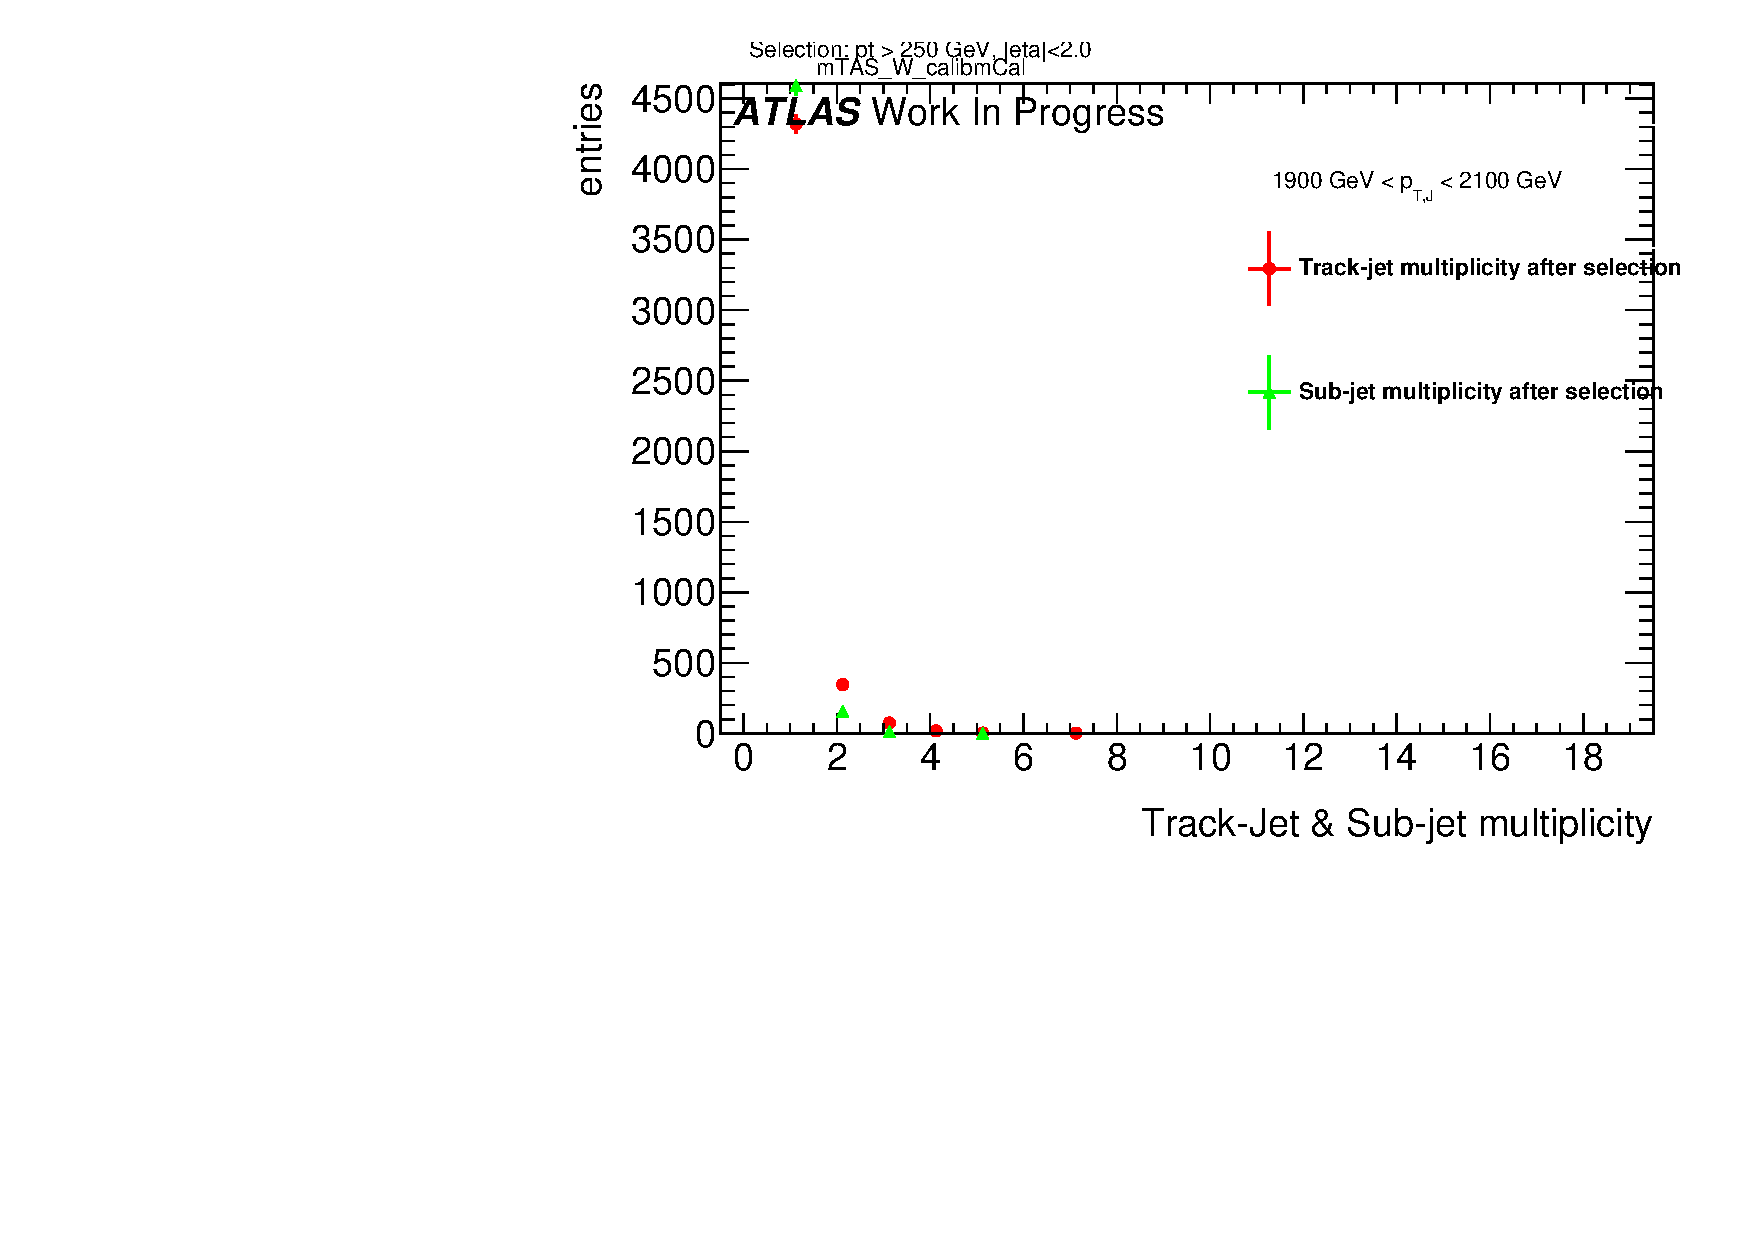
\includegraphics[width=\textwidth]{/Users/fabnap/Documents/MasterArbeit/jet_part/mta/13cfrt_h_SubJet_aftersel_ptJ10TAmult.pdf}
   
%         \label{fig:tiger}
    \end{subfigure}
    \caption{Sub-jet and Track-jet (jets created having tracks as input) multiplicity, for selected bins of transverse momentum.} 
    \label{fig:multi}
\end{figure}


\begin{figure}
    \centering
   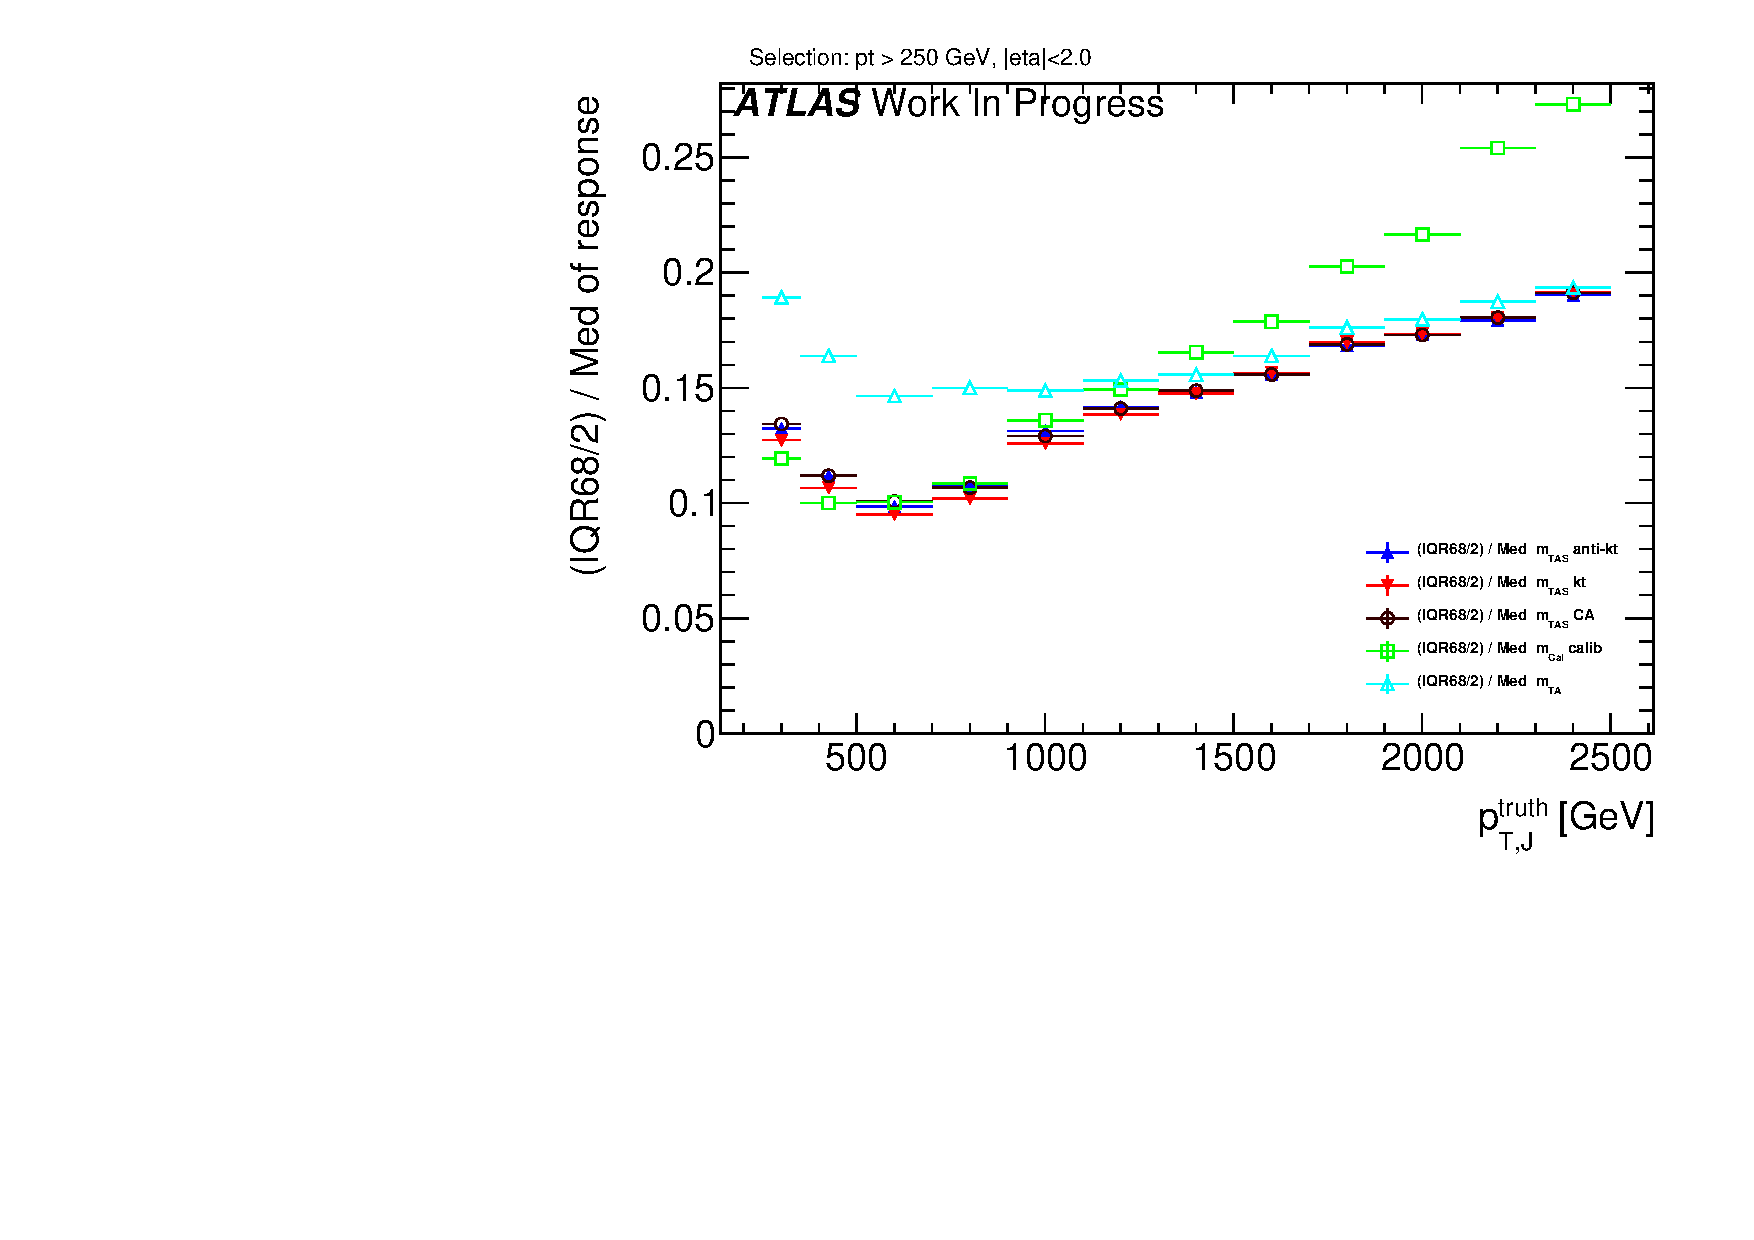
\includegraphics[width=\textwidth]{/Users/fabnap/Documents/MasterArbeit/jet_part/mtas/71graphcftr_h_JetRatio_mJ12CALOIQRoM_Wprime_Allalgos.pdf}
   
    \caption{Performance of $\mtas$ with different reclustering algorithm for the sub-jets: anti-k$_t$, k$_t$ and C/A. Boosted $W/Z$ sample.}
    \label{fig:allalgow}
\end{figure}

\begin{figure}
    \centering
   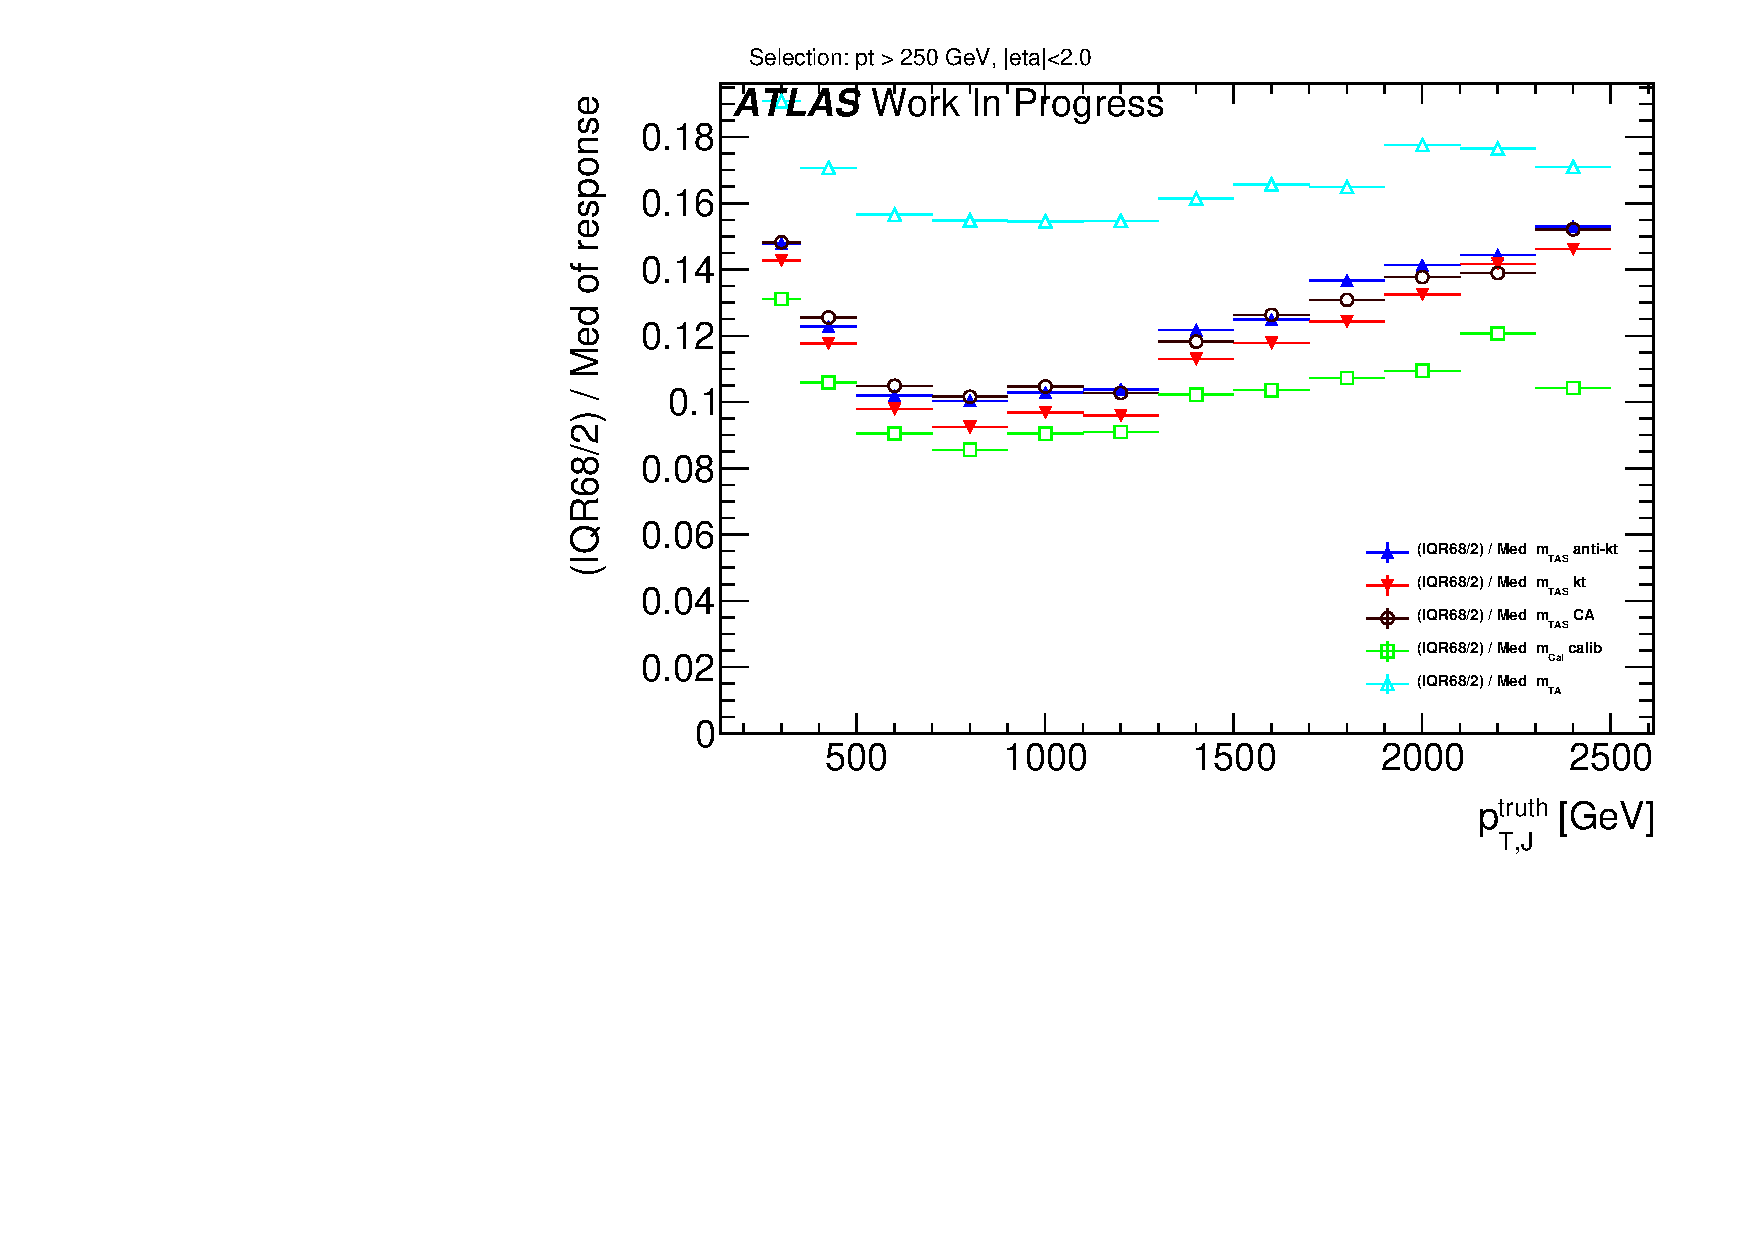
\includegraphics[width=\textwidth]{/Users/fabnap/Documents/MasterArbeit/jet_part/mtas/71graphcftr_h_JetRatio_mJ12CALOTopsCalib.pdf}
   
    \caption{Performance of $\mtas$ with different reclustering algorithm for the sub-jets: anti-k$_t$, k$_t$ and C/A. Boosted top sample.}
    \label{fig:allalgotop}
\end{figure}

\begin{figure}
    \centering
   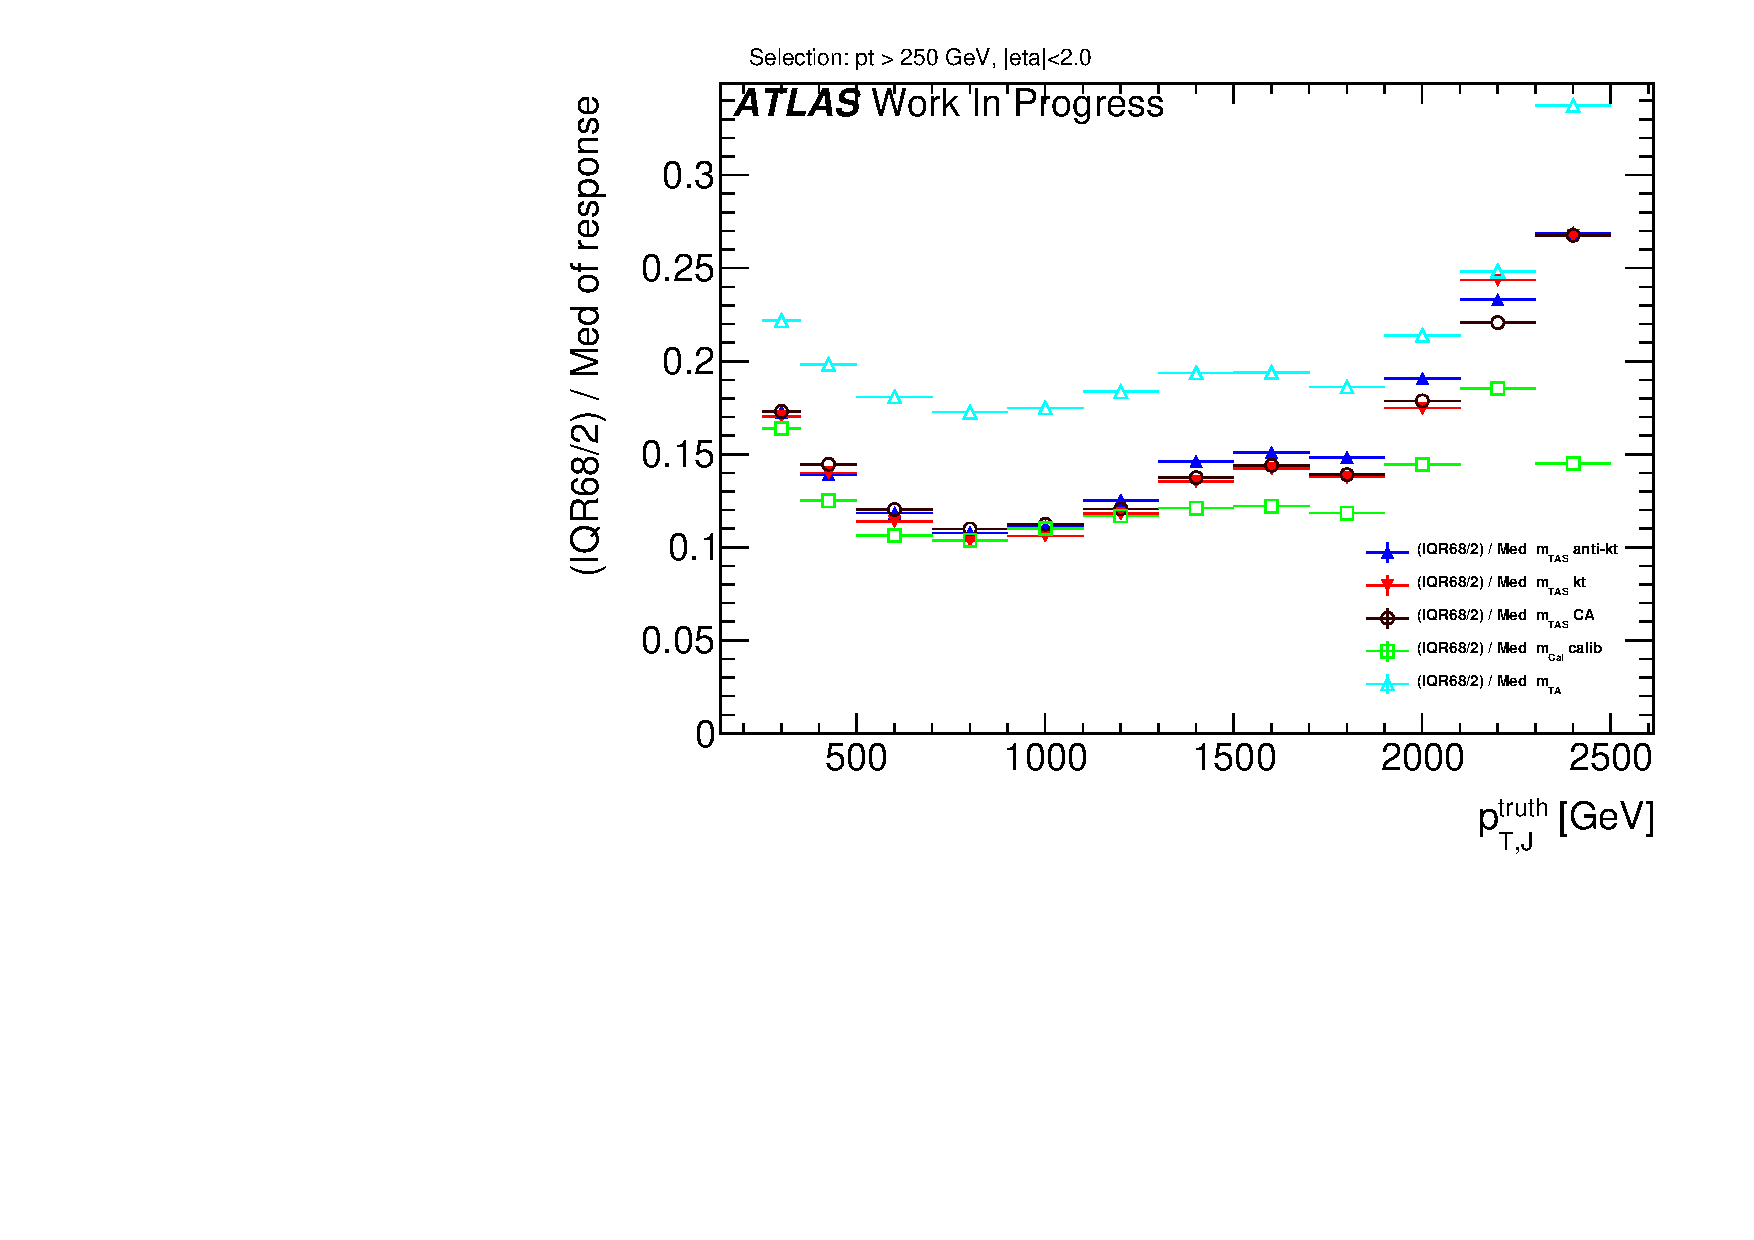
\includegraphics[width=\textwidth]{/Users/fabnap/Documents/MasterArbeit/jet_part/mtas/71graphcftr_h_JetRatio_mJ12CALOIQRoMHiggsNOCalib.pdf}
   
    \caption{Performance of $\mtas$ with different reclustering algorithm for the sub-jets: anti-k$_t$, k$_t$ and C/A. Boosted higgs sample.}
    \label{fig:allalgohiggs}
\end{figure}


\begin{figure}
    \centering
    \begin{subfigure}[b]{0.5\textwidth}
	\centering
        \includegraphics[width=\textwidth]{/Users/fabnap/Documents/MasterArbeit/jet_part/mta/mTA_WZ/1cfrt_h_fabsca_tascal_2.pdf}
%         \rlap{\crule[white]{1cm}{1cm}}
	\put(-35,04){\crule[white]{0.15cm}{0.15cm}}
%         \label{fig:mcomba1}
    \end{subfigure}
    \begin{subfigure}[b]{0.5\textwidth}
	\centering
        \includegraphics[width=\textwidth]{/Users/fabnap/Documents/MasterArbeit/jet_part/mta/mTA_Tops/1cfrt_h_fabsca_tascal_2.pdf}
	\put(-35,04){\crule[white]{0.15cm}{0.15cm}}
%         \label{fig:mcomba2}
    \end{subfigure}
    
    \begin{subfigure}[b]{0.5\textwidth}
	\centering
        \includegraphics[width=\textwidth]{/Users/fabnap/Documents/MasterArbeit/jet_part/mta/mTA_higgs/1cfrt_h_fabsca_tascal_2.pdf}
	\put(-35,04){\crule[white]{0.15cm}{0.15cm}}
%         \label{fig:mcomba3}
    \end{subfigure}
    
    \caption{Calorimeter based jet mass response vs the track-assised mass response for the three signal samples. Correlation coefficient is indicated on the top right.} 
    \label{fig:mcomba1}
\end{figure}


\begin{figure}
    \centering
   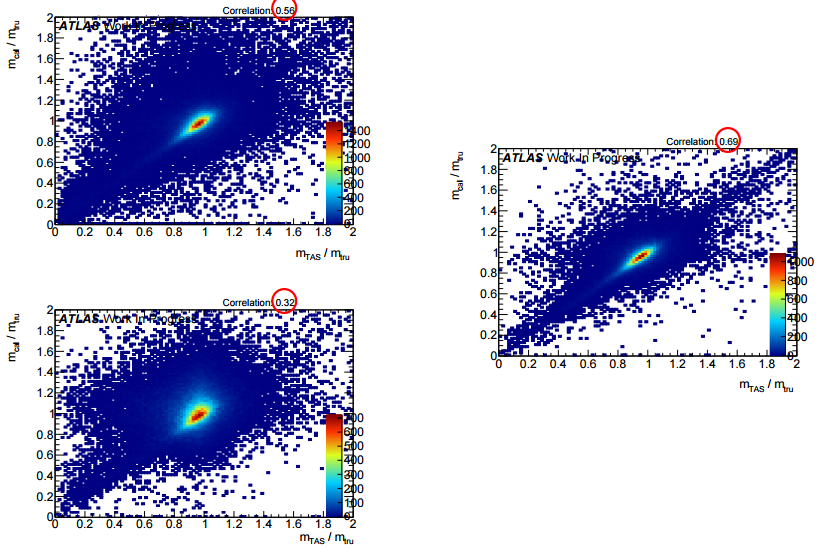
\includegraphics[width=1.2\textwidth]{/Users/fabnap/Documents/MasterArbeit/jet_part/mcomb/mcomba2.png}
    \caption{Calorimeter based jet mass response vs the track-assised sub-jet mass response for the three signal samples. Correlation coefficient is indicated on the top right and highlighted.
    On the left, top, the higgs sample, bottom, the $W/Z$; on the right the top-quark sample.}
    \label{fig:mcomba2}
\end{figure}


\begin{figure}[!ht]
  \centering
      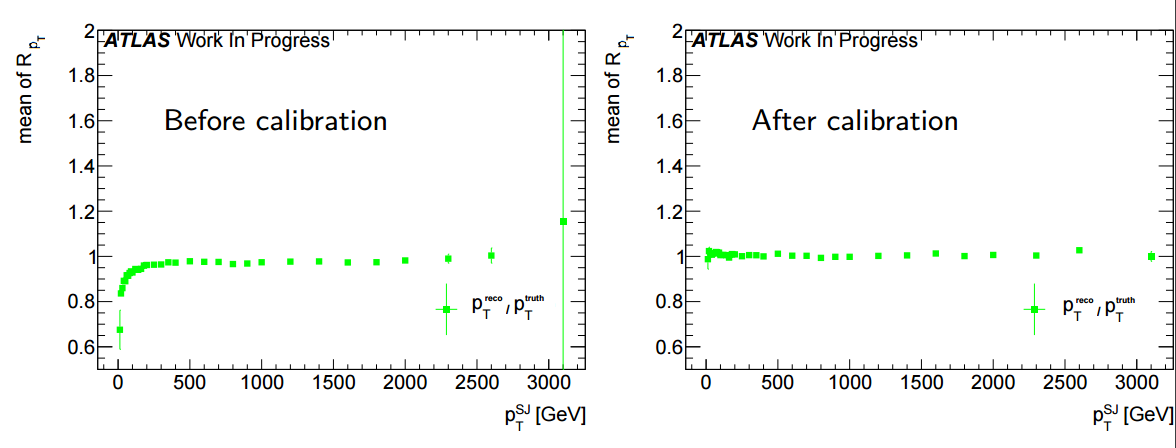
\includegraphics[width=\textwidth]{/Users/fabnap/Documents/MasterArbeit/jet_part/calib/perfectcalib2.png}
  \caption{Poor's man calibration effect on mean of transverse momentum's response of the sub-jet, before, left, and after, right, the procedure.}
  \label{fig:calibA}
\end{figure}

\begin{figure}[!ht]
  \centering
      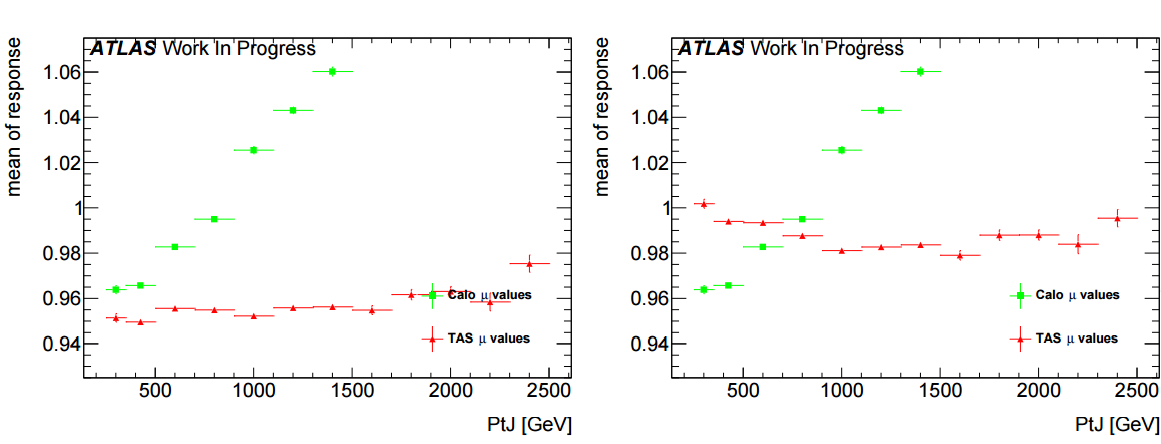
\includegraphics[width=\textwidth]{/Users/fabnap/Documents/MasterArbeit/jet_part/calib/perfectcalib3.png}
  \caption{Poor's man calibration effect on the mean of the mass response of the large-R jet, before, left, and after, right, the procedure.}
  \label{fig:calibA2}
\end{figure}


\begin{figure}[!ht]
  \centering
      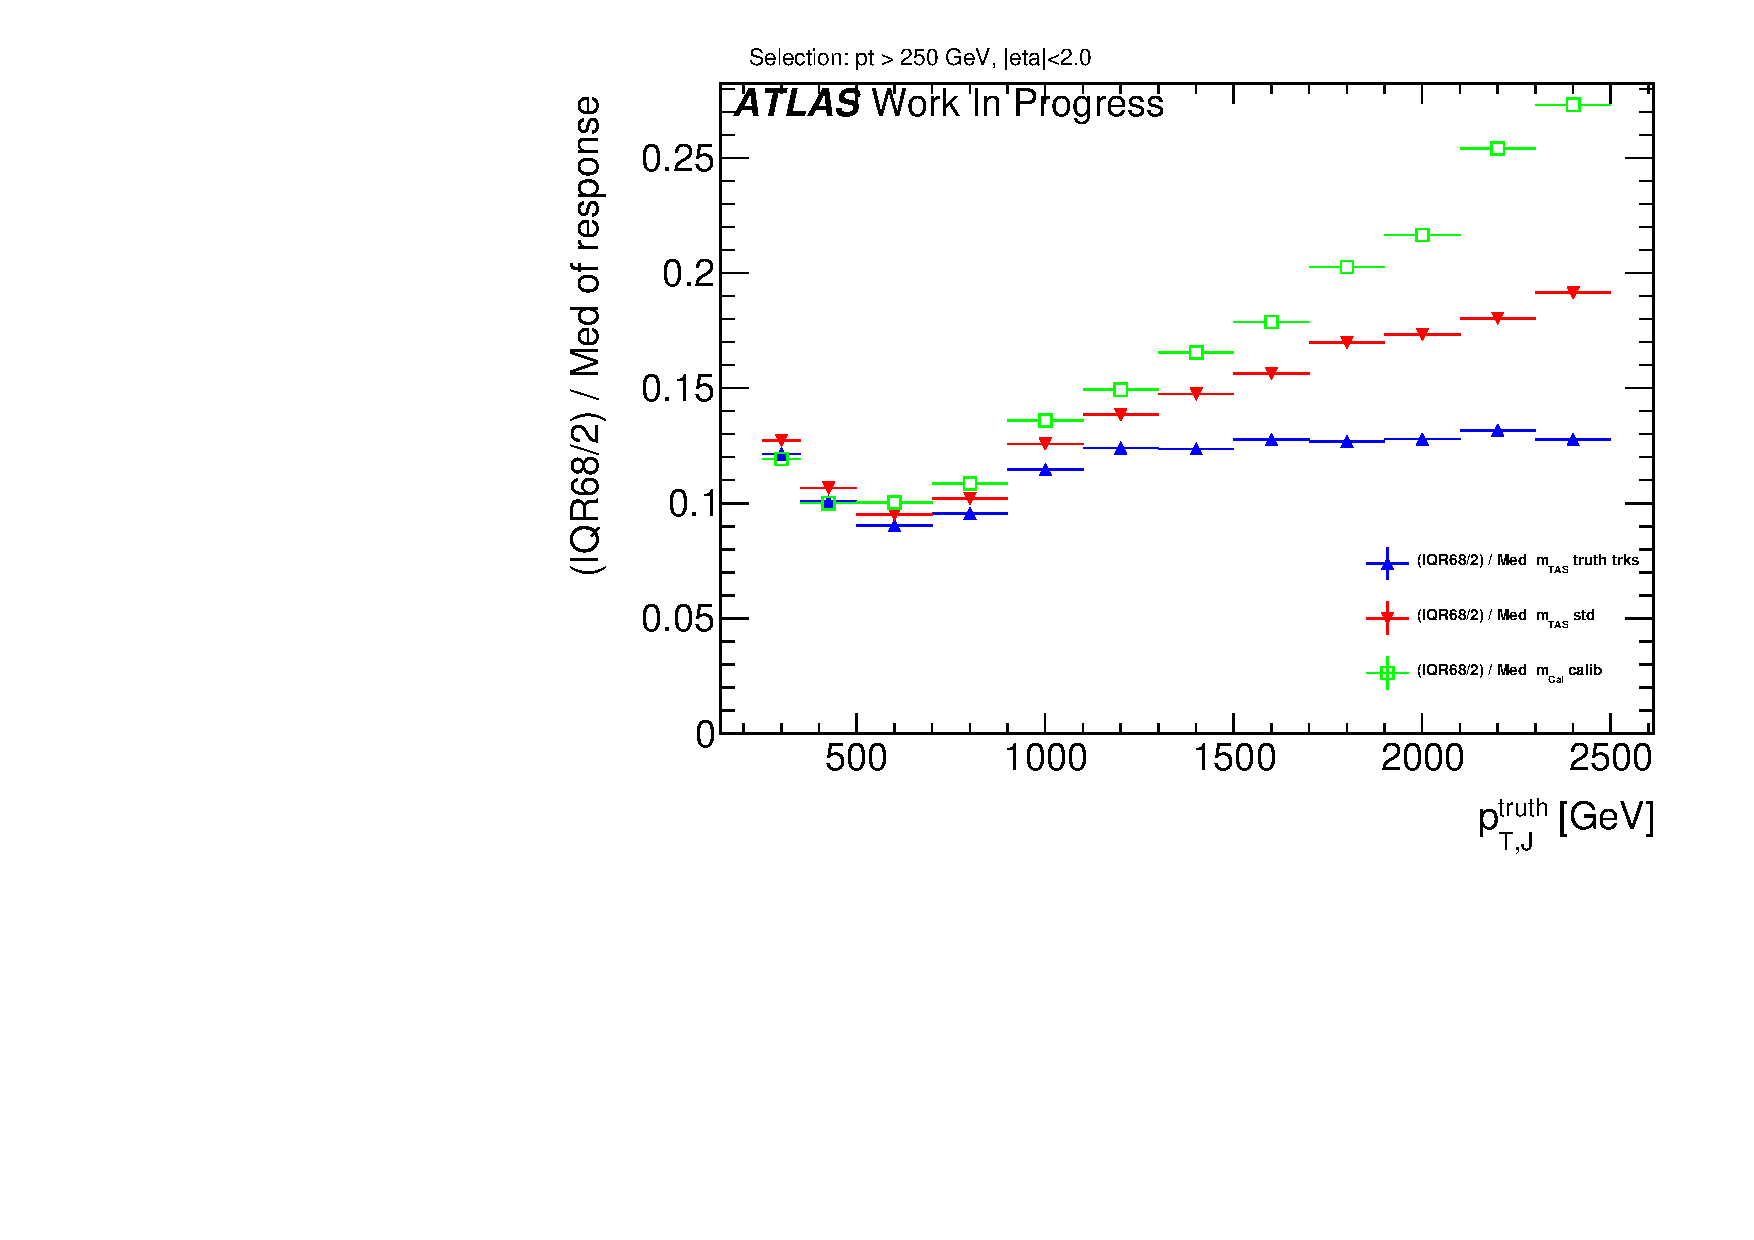
\includegraphics[width=\textwidth]{/Users/fabnap/Documents/MasterArbeit/jet_part/calib/71graphcftr_h_JetRatio_mJ12CALOIQRoMcalib_degradW.pdf}
  \caption{Comparison of the $\mtas$ and the same variable using truth-level information for the tracks.}
  \label{fig:breakdown1}
\end{figure}